
Proposed system aims to make a machine learning model which could predict the real estate house prices. Respective chapter has in view of the content focusing on scope, motivation, objectives and selection of life cycle model of the projected system. It also states the actual problem definition which is to be solved using machine learning models .\\
The Section 1.1 describes the background of the promised proposed system to be built. Motivation behind selecting particular problem statement is presented in section 1.2. The section 1.3 discuss about the problem definition. The scope of the system is discussed in section 1.4. The section 1.5 discuss about objectives of proposed system. The selection of life cycle model for development of system is discussed in section 1.6. The section 1.7 will discuss about organization of report. Finally, the summary is presented in the last section.

\section{Background}
% Content inside the background section

\section{Motivation}
% Content inside the motivation goes here
Being extremely interested in everything having a relation with the Machine Learning, the final year project was a great occasion to devote time to learn and confirm the interest for this field. The fact that machine learning can make estimations, predictions and give the ability for machines to learn by themselves is both powerful and limitless in terms of application possibilities.\\
Machine learning can be used in finance, medicine, almost everywhere. Hence that is the pivotal motivation of carrying out the final year project around machine learning domain.




\section{Problem Definition}
% Content of the problem definition goes here
In India, there are multiple real estate classified websites where properties are listed for sell/ buy/ rent purposes such as 99acres, housing, commonfloor, magicbricks and more. However, in each of these websites we can see lot of inconsistencies in terms of pricing of an apartment and there are some cases when similar apartments are priced differently and thus there is lot of in-transparency. Sometimes the consumers may feel the pricing is not justified for a particular listed
apartment but there no way to confirm that either. Proper and justified prices of properties can bring in a lot of transparency and trust back to the real estate industry, which is very important as for most consumers especially in India the transaction prices are quite high and addressing this issue will help both the customers and the real estate industry in the long run. We propose to use machine learning and artificial intelligence techniques to develop an algorithm that can predict housing prices based on certain input features.\\
The business application of this algorithm is that classified websites can directly use this algorithm to predict prices of new properties that are going to be listed by taking some input variables and predicting the correct and justified price i.e. avoid taking price inputs from customers and thus not letting any error creeping in the system. This study on proactive pricing of houses in the Indian context has never been reported earlier in the literature to the best of our knowledge.\\
However, the problem of house price prediction is quite old and there have been many studies and competitions addressing the same including the classic Boston housing price challenge on Kaggle. As far as housing price prediction in Indian context is concerned, use of machine learning algorithm can really get the job done.




\section{Scope}
\section{Objective}

\section{Selection of Life Cycle Model for Development}
% Content inside the selection of life cycle model

In order to accomplish the stated objective, Agile model is selected as software development life cycle model. The incentive behind selecting Agile model is because requirements
are stated clearly but the machine learning model needs to be trained and tested for better prediction on unseen data which makes the implementation and testing phase repetitive.
\begin{figure}[!ht]
\centering
        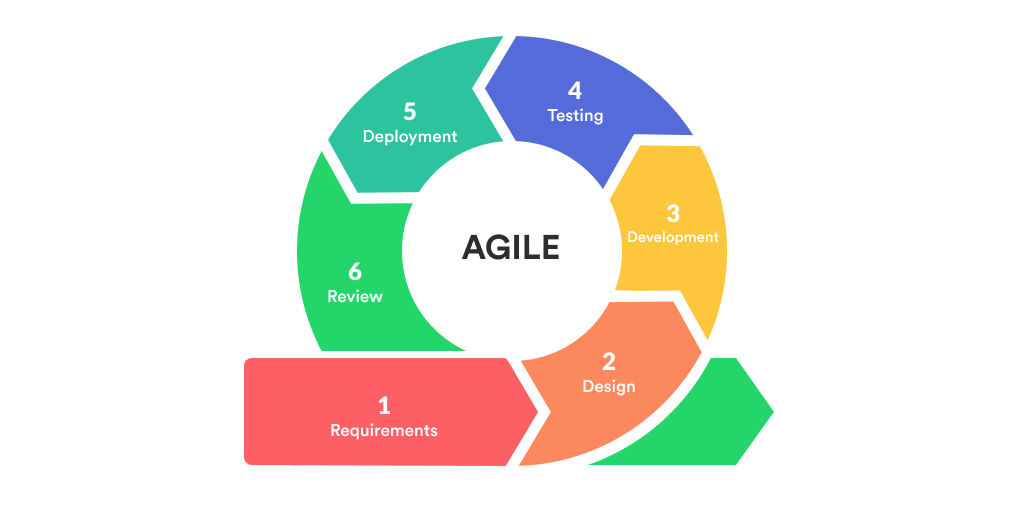
\includegraphics[totalheight=8cm]{Introduction/AgileModel.png}
    \caption{Software Development Life Cycle Model}
    \label{fig:verticalcell}
\end{figure}


\section{Organization of Report}
% Content inside the organization of the report goes here

Chapter 1: Chapter 1, Problem definition of the proposed machine learning model is given along with background history, motivation for developing this system. Scope and objective of projected system is discussed.\\ 
Chapter 2: Chapter 2, will talk about literature referred for getting this idea of project design. Actual working and functionalities of the proposed machine learning model is described here. Section 2.1 will be brief about economical, operational and technical feasibility of the given system. Risk analysis is done in section 2.2 along with planning and effort allocation for development of proposed system in section 2.3 and 2.4.\\
Chapter 3: Chapter 3, will discuss about requirements of machine learning model. Hardware as well as software requirements are described in section 3.1 and section 3.2. Section 3.3 will give functional and non functional requirements of the the model. And software requirements specification is stated in section 3.4.\\
Chapter 4: Chapter 4 will give pictorial representation of the system. Section 4.1 will show architecture of the machine learning model using simple block diagram. Section 4.2 will give data flow diagrams (DFDs). UML diagrams of the proposed system are given in section 4.3.\\
Chapter 5: In chapter 5, conclusion about whatever work had done is discussed in section 5.1. Future work are discussed in section 5.2. At the last, project report embody bibliography too.


\section{Summary}
% Content of the summary section goes here
The given chapter thoroughly describes background and motivation behind selecting this machine learning project. The problem definition, scope and objective are also stated in the given chapter. The organization of report gave the overall structure about the chapters described throughout in this report upfront. The next chapter will discuss about system analysis.
